% Chapter 3 (from main tex file)
% New Trends in Research
% Author: Javier Reyes

\chapter{Vivado Design Suite}

The Vivado Design Suite is the IDE provided by Xilinx Inc. for the design and development with their FPGA products and solutions. As part of the tool, a IDE for software development called Xilinx SDK is also provided. A third tool bundle for embedded linux image building is available independently in Xilinx web site, but that keeps strong relation to the Vivado program.

\section{Installation}

The main procedure for the installation of the Xilinx development platform is described in the UG973\footnote{Vivado Design Suite User Guide, Release Notes, Installation and Licensing v2017.4}. The tools are available for Windows, as well as most GNU-Linux OS. For the scope of this project, it is highly recommended to use Linux, considering that the hardware requirements are considerable high for a standar desktop PC, and also the image building tool runs \underline{only} on Linux.

The Vivado installer can be downloaded directly from the Xilinx downloads page. This web installer includes the Vivado Design Suite for Hardware Description and the Xilinx Software Development Kit (SDK) for software (standalone and embedded) development. The installer will trigger the download of the necessary files on the web, which can vary from 5 to 7 GB depending on the installation options.

In order to install the Vivado Suite on a secure location (under linux file systems the folder \texttt{/opt} is recommended), the installer should be executed with root privileges, despite the fact that the official documentation claims that it can be run without them. The linux installer also requires that the USB cable drivers are installed after the Suite installation (not necessary in Wondows, as this installer is executed automatically). The following script can be used as a guide for the installation:

\begin{lstlisting}[language=bash, basicstyle=\scriptsize\ttfamily, tabsize=2, commentstyle=\color{darkgray}, keywordstyle=\color{blue}, backgroundcolor=\color{lightgray}, morekeywords={chmod, sudo}, numbers=left, breaklines=true]
	# Give executable permission to the installer file
	chmod +x <installer_filename>.bin
	# Executes the installer with root privileges
	# Select the WebPack edition - no cost
	# Include at least the SDK and the device Zynq in the content selection
	# Select the installation folder
	sudo ./<installer_filename>.bin
	# After install, change to the driver cable installer folder
	cd <vivado_folder>/data/xicom/cable_drivers/lin64/install_script/install_drivers/
	# Execute the driver cable installer with root privileges
	sudo ./install_drivers
	# Create the apropiate environment for the suite to be launched
	# Needs to be run everytime before launching Vivado
	# Alternatively, can be added to the .bashrc to be executed automatically
	source _vivado_installed_folder_/settings64.sh
	# Launch the Vivado GUI, blocks the terminal when launched
	vivado &
\end{lstlisting}

\section{Project Configuration}

Once the Vivado Design Suite is installed and running, the hardware project can be created. The GUI launches a wizard that allows to select the folder for the project (this folder will also contain the software projects from SDK), the type of Xilinx project (RTL) and the device (as shown in the figure \ref{fig:device-vivado}).

\begin{figure}[h!]
	\centering
	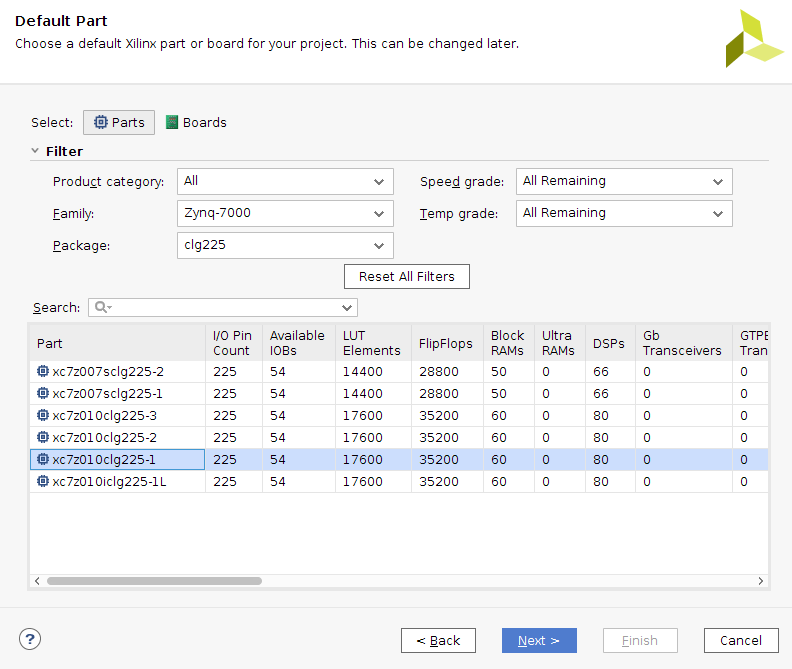
\includegraphics[width=0.7\textwidth]{project-device.png}
	\caption{Device selection - Xilinx Hardware Project.}
	\label{fig:device-vivado}
\end{figure}

The hardware definition for the Zynq-7000 family implies the use of an IP Core design provided by Xilinx, in order to use the embedded ARM Cortex processor. Additional IP Cores can be added to the design in the Programmable Logic section, or user-defined hardware definition modules can be included.

The procedure for the hardware definition can vary depending on the specific hardware, and the requirements that the final application presents. A general procedure can be found in the User Guide UG1165\cite{UG1165}.

\begin{enumerate}
	\item Create a new Block Design.
	\item Add the Zynq7 Processing System IP Core to the Block Design.
	\item Add/create all the necessary HDL modules or IP Cores [Optional].
	\item Configure the Zynq7 PS Core:
	\begin{enumerate}
		\item Apply the configuration in a TCL script file (provided by the manufacturer), or manually configure the Core in the GUI.
		\item Ensure that the necessary peripherals are enabled (CAN, USB).
		\begin{figure}[h!]
			\centering
			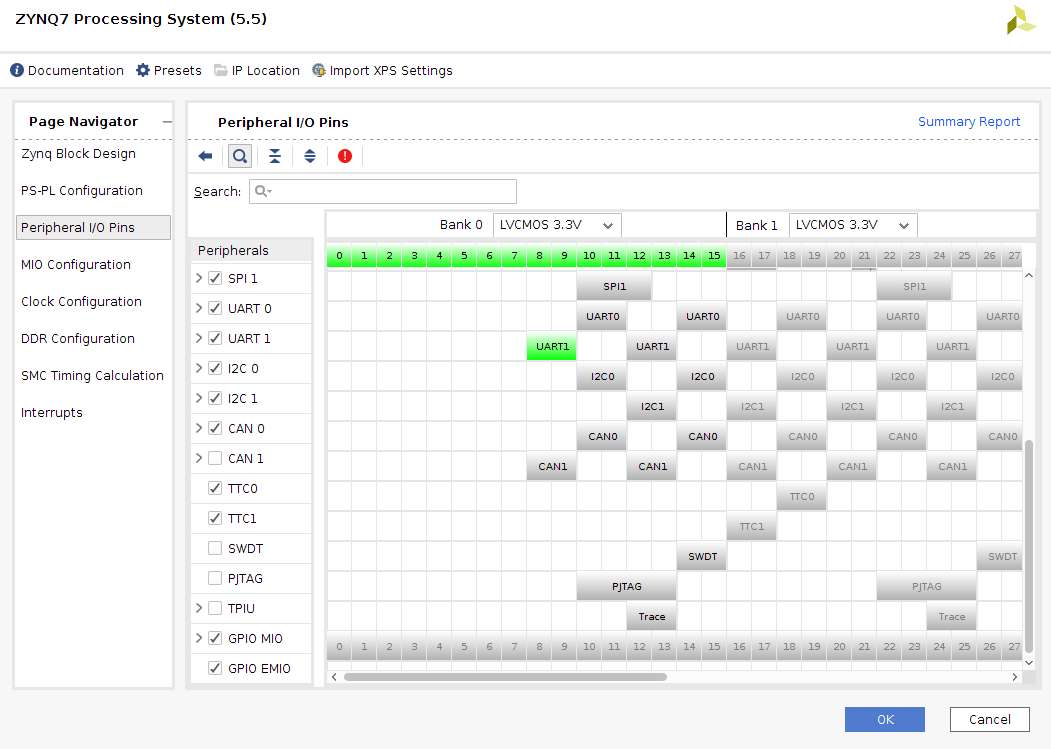
\includegraphics[width=0.7\textwidth]{can-enable.png}
			\caption{CAN peripheral enable.}
			\label{fig:can-enable}
		\end{figure}
		\item Ensure that the modules that are enabled (not by default) are routed to an available MIO pin (see Trenz TRM \cite{zynq-trm}), or via EMIO.
		\begin{figure}[h!]
			\centering
			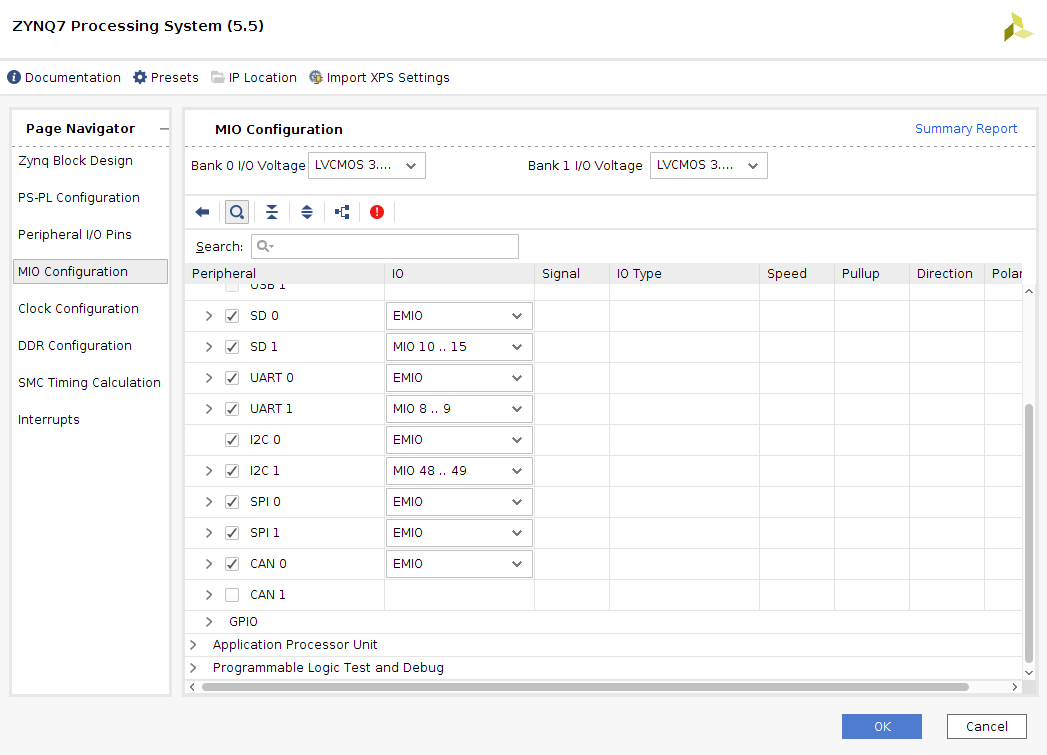
\includegraphics[width=0.7\textwidth]{can-emio.png}
			\caption{CAN signals routing through EMIO.}
			\label{fig:can-emio}
		\end{figure}
		\item Configure the frequency for the CAN REF CLK signal (80MHz)\footnote{The default value is 100Mhz, but in lab tests the CAN timing was imperfect with this setting, while 80Mhz produce an exact time quanta for the 500 kbps CAN network.}.
		\begin{figure}[h!]
			\centering
			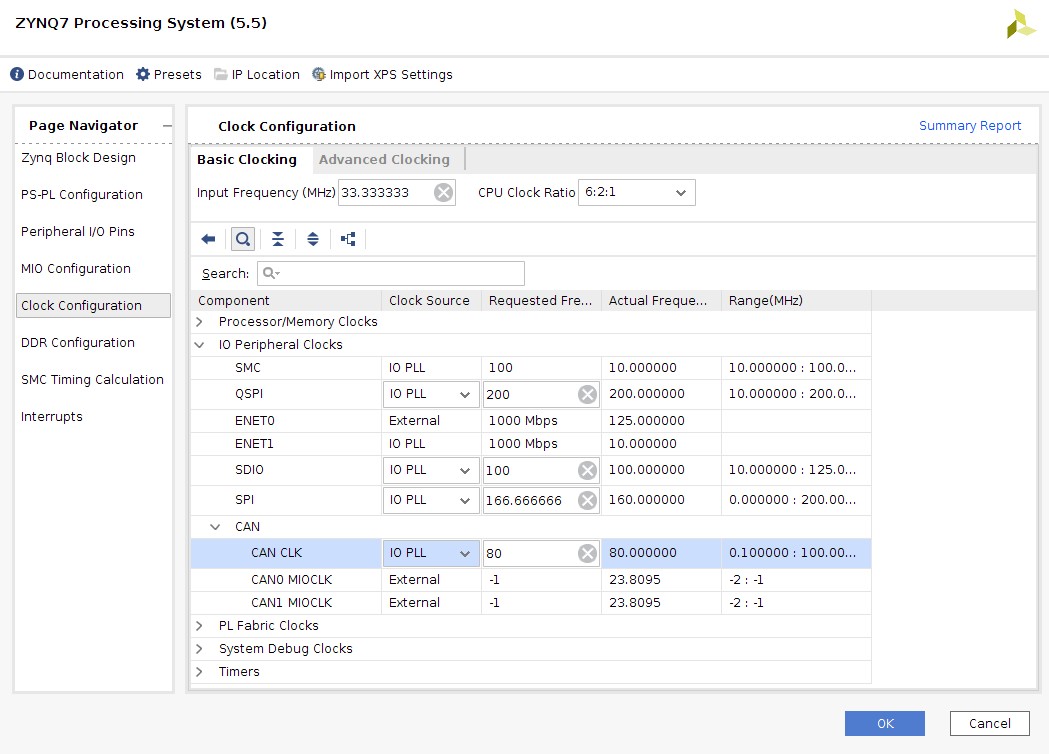
\includegraphics[width=0.7\textwidth]{can-clock.png}
			\caption{CAN module reference clock configuration.}
			\label{fig:can-clock}
		\end{figure}
	\end{enumerate}
	\item Run the Block Automation wizard.
	\item Run the Connection Automation wizard.
	\item Config all the signals that will be routed to a physical pin external (Make external).
	\begin{figure}[h!]
		\centering
		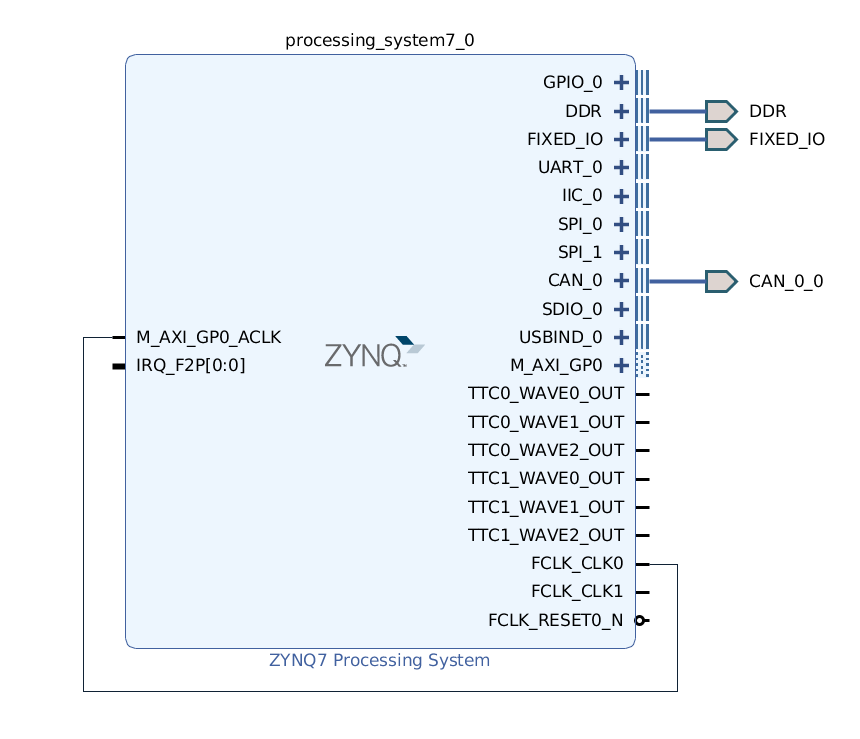
\includegraphics[width=0.7\textwidth]{ip-core.png}
		\caption{IP Core design block ready to sinthetize.}
		\label{fig:ip-core}
	\end{figure}
	\item Generate an HDL wrapper for the Block Design.
	\item Open the Elaborated Design (RTL Analysis), and set the I/O planning layout.
	\item Config the IO standard (LVCMOS33 for the Zynqberry board) and package pin for the signals made external (see Trenz TRM \cite{zynq-trm}).
	\item Run Synthesis, Implementation and Generate Bitstream.
	\item Export hardware, including bitstream file.
	\item Launch SDK, selecting the local project environment.
\end{enumerate}

At this point, the SDK will be started and automatically imported the hardware definition file. From this point, the software can be designed for this specific implementation.

The Vivado tool is also capable of command line scripts in TCL scripting language. This method can be a quite more complex to follow than the GUI, but it also increases the certainty in the procedure, as well as the ease of share, debug or collaborate (as a text file, can be easily pushed into a Source Control repository). The repository contains a file \texttt{create\_project.tcl} (snippet shown partially), that can recreate the workflow above defined if run from the Xilinx Vivado TCL console \cite{UG835}.

\lstinputlisting[language=tcl, basicstyle=\scriptsize\ttfamily, tabsize=2, commentstyle=\color{darkgray}, keywordstyle=\color{blue}, backgroundcolor=\color{lightgray}, morekeywords={create_project}, firstline=1, lastline=10, breaklines=true, numbers=left]{../../../git/DAEbot/Devices/Zynqberry_OperatorPlus/zynqberryHW_CAN/create_project.tcl}

\section{IDiAL Server}

In order to keep the environment available for further development, a Virtual Machine has been created in the IDiAL Server from FB4, with the following characteristics:

\begin{itemize}
	\item VM: U16x64D\_Vivado
	\item User: Javier
	\item Password: IDiAL
	\item OS: Ubuntu 16.04.3 Desktop
	\item IP-Address: 172.22.167.120
\end{itemize}

On this machine, the Vivado Design Suite was installed, as well as the Petalinux tool, in order fully handle the Zynqberry device. In order to access it, the VMware client can be used in Windows, or using the \texttt{vpnc} package in Linux. It can only be accessed from the FB4 network directly, or via the FB4 VPN\footnote{Connection details under \underline{https://www.fh-dortmund.de/de/fb/4/103020100000253634.php}}
